\chapter{Relational Learning with Embeddings}

\section{Poincaré Embeddings}

% Authors: Manrique Vargas, Aakriti Gupta, HuiYu Sun
% Part 2
% Lecture date: 4/22/2019

\subsection{Introduction}
We introduce hierarchical representations of symbolic data by embedding them into hyperbolic space – an n-dimensional Poincaré ball. The underlying hyperbolic geometry allows us to learn representations of symbolic data by simultaneously capturing hierarchy and similarity\cite{NIPS2017_7213}. The underlying hyperbolic geometry allows us to learn representations of symbolic data by simultaneously capturing hierarchy and similarity. We present an efficient algorithm to learn the embeddings based on Riemannian optimization and show experimentally that Poincaré embeddings can outperform Euclidean embeddings significantly on data with latent hierarchies, both in terms of representation capacity and in terms of generalization ability .

\subsection{Poincaré Model of Hyperbolic Space}

Poincaré Model of Hyperbolic Space can embed data such that the distance in the embedding space reflects their semantic similarity. It assumes that there exists a latent hierarchy in which the symbols can be organized. In addition to the similarity of objects, it intends to reflect this hierarchy in the embedding space to improve over existing methods in two ways:
\begin{itemize}
    \item Incorporate an appropriate structural bias on the embedding space to improve generalization performance, run time, and memory complexity.
    \item Capture the hierarchy explicitly in the embedding space to gain additional insights about the relationships between symbols and the importance of individual symbols.
\end{itemize}

The model considers the task of inferring the hierarchical relationships fully unsupervised, as is, for instance, necessary for text and network data. In contrast to Euclidean space $ \mathbb{R}$, there exist multiple, equivalent models of $ \mathbb{H}$ such as the Beltrami-Klein model, the Hyperboloid model, and the Poincaré half-plane model. 

Poincaré ball model is well-suited for gradient-based optimization. In particular, assume a Riemannian manifold $(B_d , d_p )$ where  $B_d = {x \in \mathbb{R}_d | \norm{x} < 1}$ is the open d-dimensional unit ball, where $\norm{}$ denotes the Euclidean norm. The distance between points $\Vec{u}$, $\Vec{v} \in B_d$ is given as:

\begin{equation} \label{eq:poincarredistance}
    d_p(\Vec{u},\Vec{v})= arcosh(1+2 \dfrac{\norm{\Vec{u}-\Vec{v}}^2}{(1-\norm{\Vec{u}}^2)(1-\norm{\Vec{v}}^2)})
\end{equation}

 The boundary of the ball is denoted by ∂B. It corresponds to the sphere S d−1 and is not part of the manifold, but represents infinitely distant points. Geodesics in B d are then circles that are orthogonal to $\delta B$ (as well as all diameters). See ~\ref{fig:poincaredisk} and ~\ref{fig:poincaregrowthdist} for an illustration.

It can be seen from Equation ~\ref{eq:poincarredistance}, that the distance within the Poincaré ball changes smoothly with
respect to the location of u and v. This adds a locality property to amplify the Euclidean distance. This locality property of the Poincaré distance is key for finding continuous embeddings of hierarchies. For example, by placing the root node of a tree at the origin of $B_d$ it would have a relatively small distance to all other nodes as its Euclidean norm is zero. On the other hand, leaf nodes can be placed close to the boundary of the Poincaré ball as the distance grows very fast between points with a norm close to one. Furthermore, please note that Equation ~\ref{eq:poincarredistance} is symmetric and that the hierarchical organization of the space is solely determined by the distance of points to the origin. Due to this self-organizing property, Equation ~\ref{eq:poincarredistance} is applicable in an unsupervised setting where the hierarchical order of objects is not specified in advance such as text and networks.

Equation ~\ref{eq:poincarredistance} allows us therefore to learn embeddings that simultaneously capture the hierarchy of objects (through their norm) as well a their similarity (through their distance). Since a single hierarchical structure can be well represented in two dimensions, the Poincaré disk ($ \mathcal{B}^2 $) is a common way to model hyperbolic geometry. The Poincaré ball ($ \mathcal{B}_d $) is used for two main reasons: first, in many datasets such as text corpora, multiple latent hierarchies can co-exist, which can not always be modeled in two dimensions. Second, a larger embedding dimension can decrease the difficulty for an optimization method to find a good embedding (also for single hierarchies) as it allows for more degrees of freedom during the optimization process. 

It can be seen that geodesics also have shortest paths through more general points. In addition, modelling tree structures in the Poincaré ball allows us to represent roots of the trees since points at the origin are relatively close to all points, and represent leafs as points at the boundary are far apart from most points. 
This gives us an exponential volume growth to model our distance.

\begin{figure}[htb]
    \begin{center}
    \begin{subfigure}[b]{0.3\textwidth}
    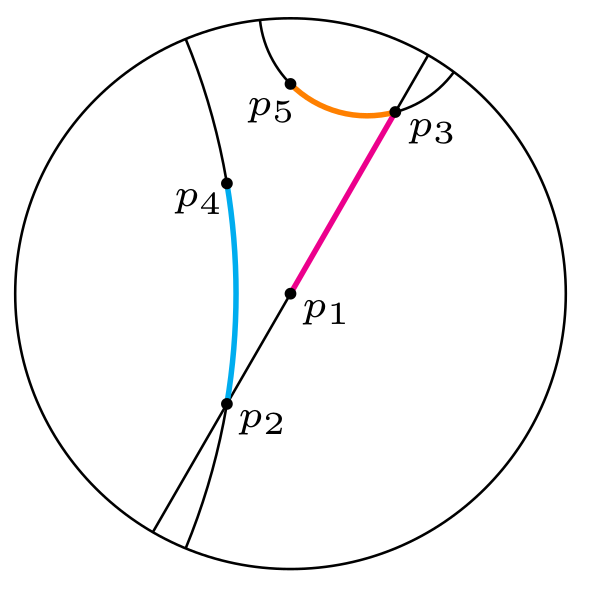
\includegraphics[width=\textwidth]{lectures/11-b/Images/1-1-1.png}
        \caption{Geodesics of the Poincaré disk}
        \label{fig:poincaredisk}
    \end{subfigure}
    \begin{subfigure}[b]{0.29\textwidth}
        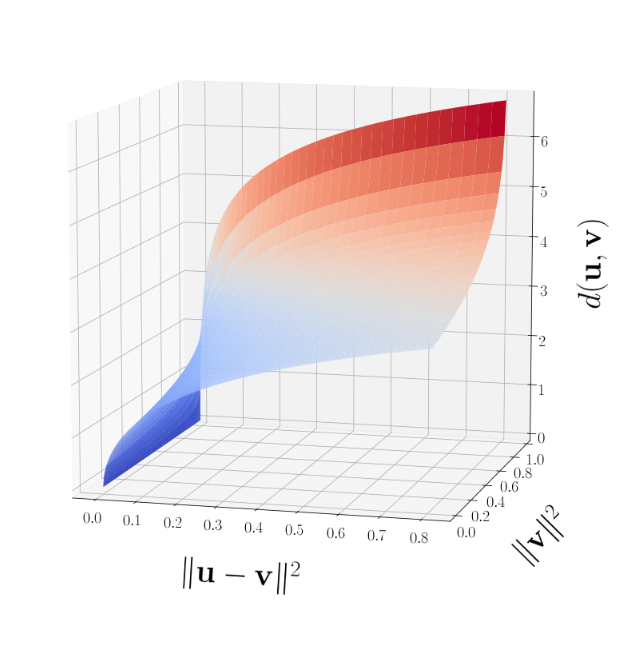
\includegraphics[width=\textwidth]{lectures/11-b/Images/1-2.png}
        \caption{Growth of Poincaré distance}       
        \label{fig:poincaregrowthdist}
    \end{subfigure}
    \caption{(a) Due to the negative curvature of B, the distance of points increases exponentially (relative to their Euclidean distance) the closer they are to the boundary. (b) Growth of the Poincaré distance $d(u, v)$ relative to the Euclidean distance and the norm of v (for fixed $\norm{u} = 0.9)$.(b) Embedding of a regular tree in $\mathcal{B} ^2$ such that all connected nodes are spaced equally far apart (i.e., all black line segments have identical hyperbolic length).}\label{fig:poincarreilus}
    \end{center}
\end{figure}

\subsection{Large Scale Embedding via Rieminian Representation}
\title{Optimization}

To compute Poincaré embeddings for a set of symbols $S = {x_i}_i^n =1$ , we are then interested in finding
embeddings $\theta = {\big\{ \theta_i\big\}}_{i=1}^n$, where $\theta_i \in  \mathscr{B}^2$ . We assume we are given a problem-specific loss function $\mathcal{L}(\theta)$ which encourages semantically similar objects to be close in the embedding space according to their Poincaré distance. To estimate $theta$, we then solve the optimization problem
\begin{equation} \label{eq:poincarresdg}
    \theta \xleftarrow{} argmin_\theta   \mathcal{L}(\theta)  s.t. \forall  \theta_i \in \theta : \norm{\theta_i} < 1
\end{equation}

As we are not in Euclidean space, we cannot use conventional stochastic gradient decent. Since the Poincaré Ball has a Riemannian manifold structure, we can optimize Equation ~\ref{eq:poincarresdg} via stochastic Riemannian optimization methods. In particular, let $\mathscr{T_\theta B}$ denote the tangent space of a point $\theta \in \mathscr{B}_d$. Furthermore, let $\nabla_\mathcal{R} \in  \mathscr{T_\theta B}$ denote the Riemannian gradient of $\mathcal{L}(\theta)$ and let $\nabla E$ denote the Euclidean gradient of $\mathcal{L}(\theta)$. Using RSGD \cite{6487381}, parameter updates to minimize Equation ~\ref{eq:poincarresdg} are then of the form:
\begin{equation} \label{eq:poincarresdg2}
    \theta_{t+1} = EXP_{\theta_t} (−\eta_t \nabla_R \mathcal{L}(\theta_t))
\end{equation}
For the minimization of Equation ~\ref{eq:poincarresdg2} we require the Riemannian gradient and a suitable retraction. Since the Poincaré ball is a conformal model of hyperbolic space, the angles between adjacent  vectors are identical to their angles in the Euclidean space. The length of vectors however might differ. To derive the Riemannian gradient from the Euclidean gradient, it is sufficient to rescale $nabla_E$ with the inverse of the Poincaré ball metric tensor, i.e. $g_/theta^{−1}$. Since $g_/theta$ is a scalar matrix, the inverse is trivial to compute. In particular, the Euclidean gradient $\nabla_E$ depends on the gradient of $\frac{\delta \mathcal{L}(\theta)}{\delta(\theta x}$, which we assume is known, and the partial derivatives of the Poincaré distance $\frac{\delta(\theta, x)}{\delta\theta}$.

Therefore we obtain the Reimannian gradient from the Euclidean gradient in the form:
\begin{equation} \label{eq:riemanniangrad}
    \nabla_{R} = g_{\theta}^{−1}\nabla_{\epsilon} = \dfrac{(1−\norm{\theta_t^2})^2}{4} \nabla_{\epsilon}
\end{equation}

Furthermore, since Equation ~/ref{eq:poincarredistance} is fully differentiable, the Euclidean gradient can easily be derived. As retraction operation, we use $Exp_{\theta}(\vec{x}) = \theta + \vec{v}$. 

Reimannian manifold has an associated Euclidean tension space. The exponential map takes the point on the tension space and takes it back to the manifold.

In summary, the full update for a single embedding is then of the form:
\begin{equation} \label{eq:riemmaniansdg}
        \theta_{t+1}  \xleftarrow{} proj \bigg(\theta_t - \eta_t\dfrac{(1−\norm{\theta_t^2})^2}{4} \nabla_E \bigg)
\end{equation}

It can be seen from that this algorithm scales well to large data-sets, as the computational and memory complexity of an update depends linearly on the embedding dimension. This model allows us to embed graphs with millions of nodes and billions of edges on a single machine.

\subsection{Evaluation of Poincare Embedding}
\subsubsection{Embedding Latent Taxonomies}

WORDNET is a lexical database that among-st others, captures hypernym relations, i.e.: 'Tiger is-a Big cat'. Embeddings trained on WORDNET provide state-of-the-art performance for lexical entailment. On collaboration networks, we show that Poincaré embeddings are successful in predicting links in graphs where they outperform Euclidean embeddings, especially in low dimensions.  

Assuming that the latent hierarchy is embedded, we can recover the latent hierarchy from indirect obfuscated graph. This way we recover the expected taxonomies and materialize the relationships. See ~\ref{fig:wn-nouns} for an illustration.
\begin{figure}[htb]
  \centering
    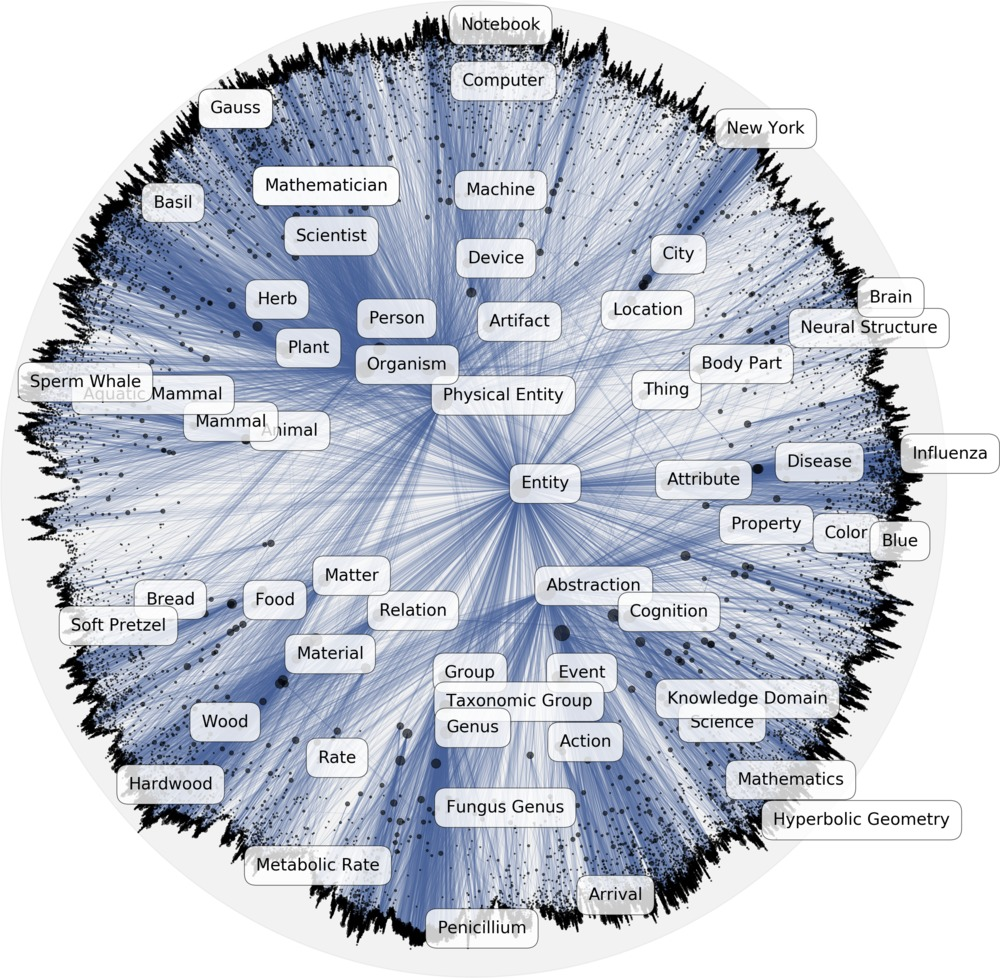
\includegraphics[width=\textwidth]{lectures/11-b/Images/wn-nouns2.jpg}
    \caption{Embedding Latent Taxonomies}
    \label{fig:wn-nouns}
\end{figure}

\subsubsection{Historical Linguistics}
Historical linguistics refer to the study of languages relations and origins. Cognates are words that are shared across different languages we assume that they indicate common entities. This example illustrates the embeddings of language in hyperbolic space. Embeddings were clustered into different language families (Roman, Germanic, Indo-European, Greek, etc.) and distance from the origin captures historical relationships. See figure  (~\ref{fig:liguistics}) for an illustration.
\begin{figure}[htb]
    \begin{center}
    \begin{adjustbox}{minipage=0.5\textwidth,scale=0.5}
    \begin{subfigure}[b]{\columnwidth}
        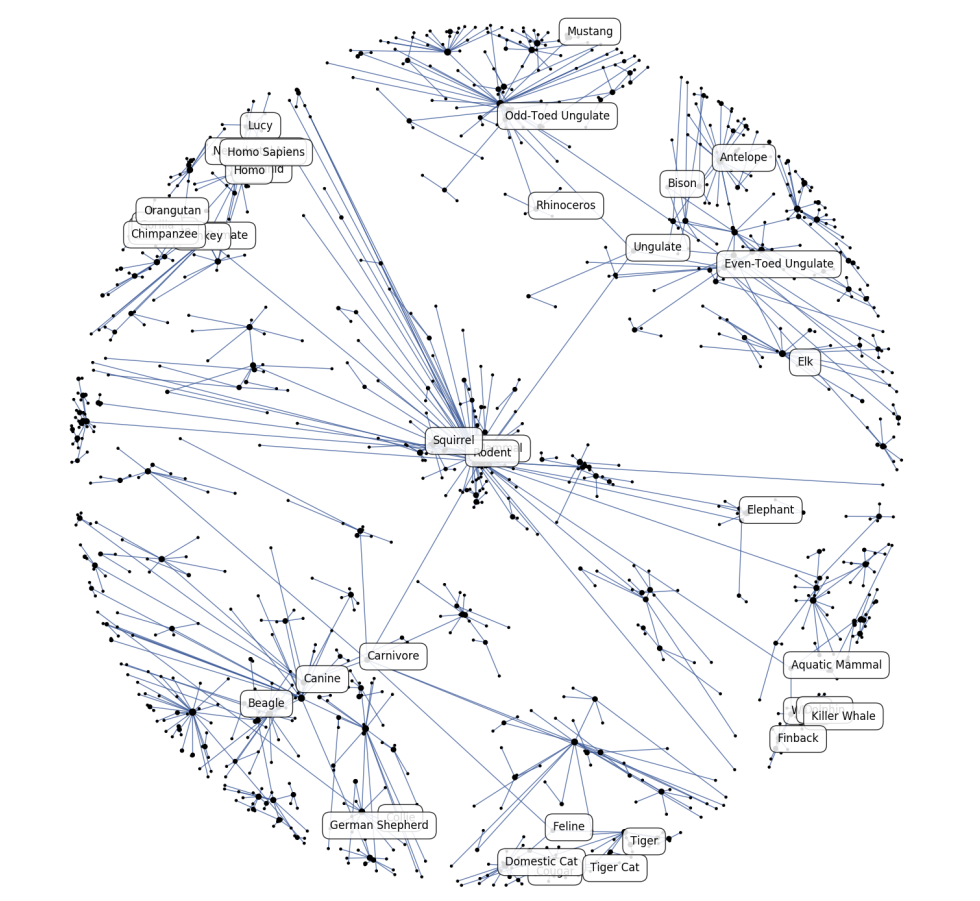
\includegraphics[width=\textwidth]{lectures/11-b/Images/1-4.png}
            \caption{Intermediate embedding after 20 epochs}
            \label{fig:linguistics1}
        \vspace{0.7cm}
        \end{subfigure}
        \begin{subfigure}[b]{\columnwidth}
            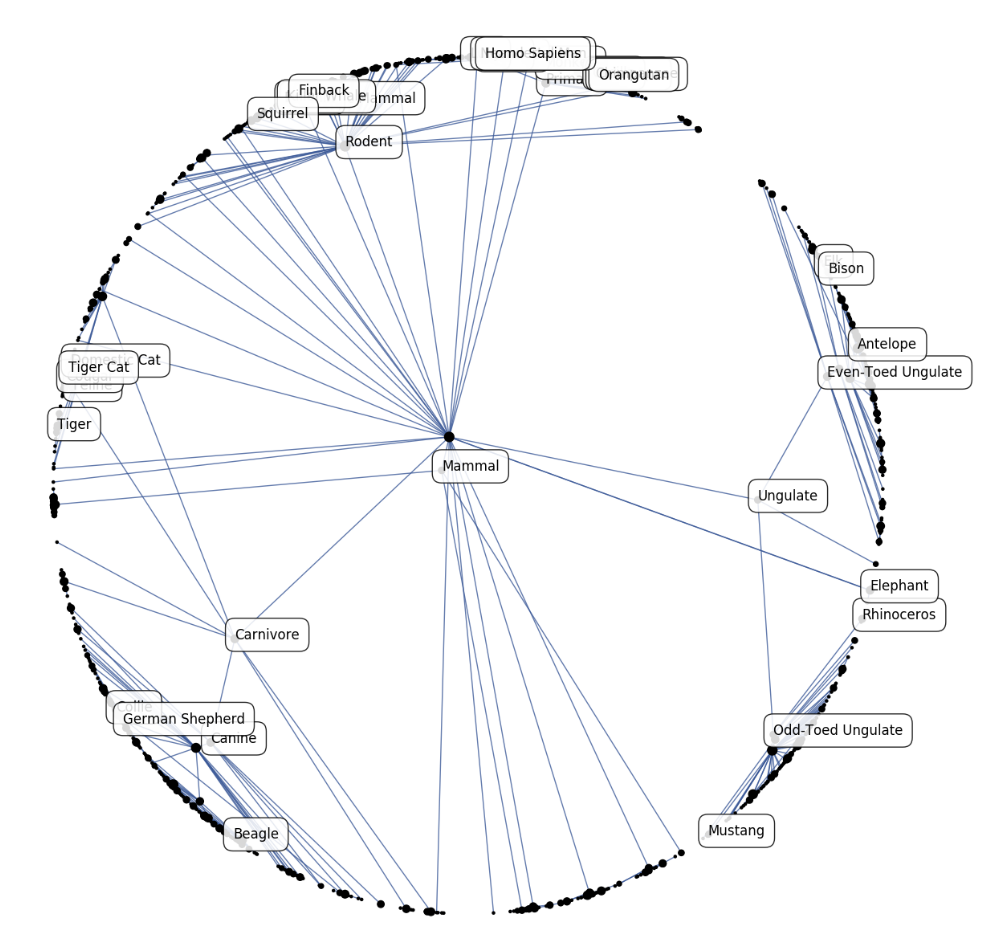
\includegraphics[width=0.5\textwidth]{lectures/11-b/Images/1-5.png}
            \caption{Embedding after convergence}       
            \label{fig:linguistics2}
        \end{subfigure}
    \end{adjustbox}
    \caption{Two-dimensional Poincaré embeddings of transitive closure of the WORDNET mammals sub tree. Ground-truth is-a relations of the original WORDNET tree are indicated via blue edges. A Poincaré embedding with d = 5 achieves mean rank 1.26 and MAP 0.927 on this subtree).}\label{fig:liguistics}
    
    \end{center}
\end{figure}

In the first set of experiments, we are interested in evaluating the ability of Poincaré embeddings to embed data that exhibits a clear latent hierarchical structure. For this purpose, Maximilian Nickel and Douwe Kiela \cite{NIPS2017_7213} conduct experiments on the transitive closure of the WORDNET noun hierarchy in two settings:
\begin{itemize}

    \item \textbf{Reconstruction.} To evaluate representation capacity, they embed fully observed data and reconstruct it from the embedding. The reconstruction error in relation to the embedding dimension is then a measure for the capacity of the model.
    \item \textbf{Link Prediction.} To test generalization performance, they split the data into a train, validation and test set by randomly holding out observed links. The validation and test set do not include links involving root or leaf nodes as these links would either be trivial or impossible to predict reliably.
\end{itemize}

Embedding based on the Poincaré distance are compared with two distance function models: Euclidean and Translational. Results are shown in table ~\ref{table:table-comparisons}:

\begin{table}[htb]
  \centering
    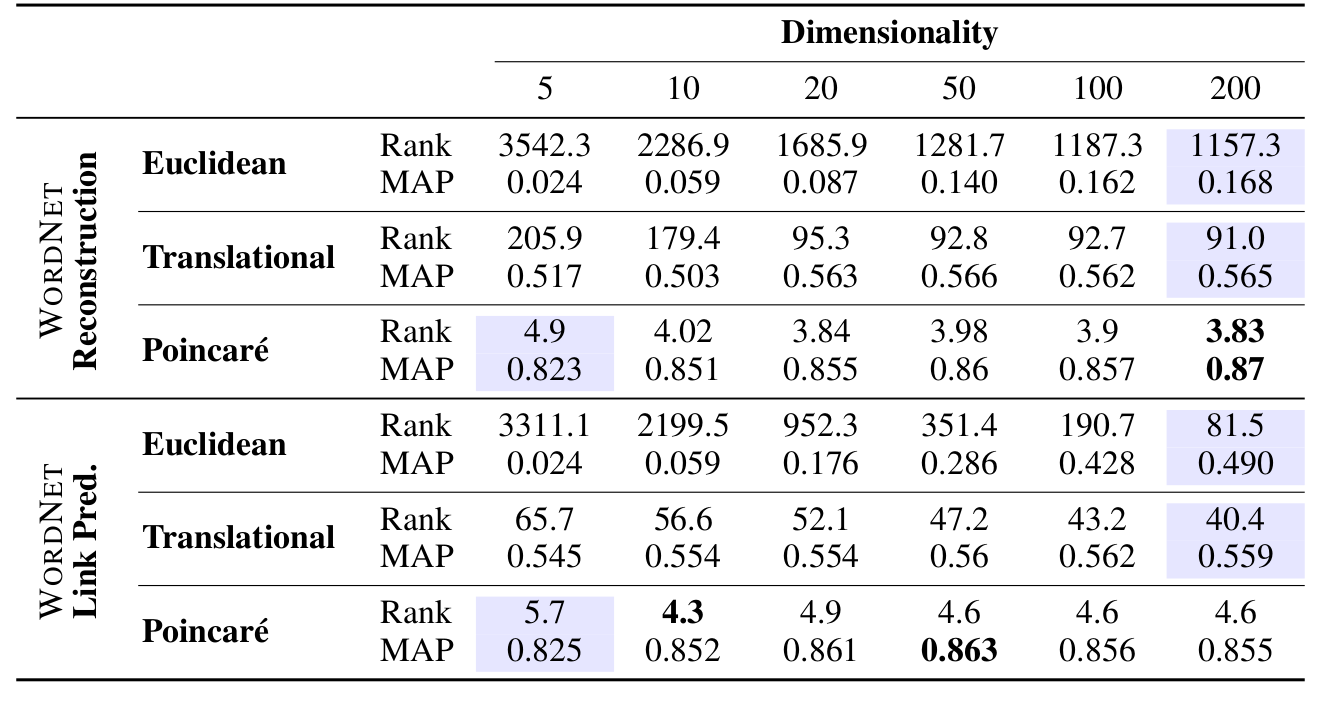
\includegraphics[width=\textwidth]{lectures/11-b/Images/1-3.png}
    \caption{Experimental results on the transitive closure of the WORDNET noun hierarchy. Highlighted cells indicate the best Euclidean embeddings as well as the Poincaré embeddings which achieve equal or better results. Bold numbers indicate absolute best results}
    \label{table:table-comparisons}
\end{table}

It can be observed from table  ~\ref{table:table-comparisons} that hyperbolic Poincaré embeddings achieve much more efficient representation for low dimensions. 

\section{Lorentz Model of Hyperbolic Space}

There are multiple equivalent models of hyperbolic space (e.g. Minkowski, Poincare, Beltram, Klein) and we can map freely between them. Lorentzian Scalar Product is an example convenient to optimize:
\begin{equation} \label{eq:riemmaniansdg3}
         \langle \vec{u},\vec{v} \rangle = -v_0 u_0 + \sum_n v_n u_n
\end{equation}  
The Hyperboloid space 
\begin{equation} \label{eq:riemmaniansdg4}
         \mathbb{H}_n = {x \in \mathbb{R}_{n+1}:\langle \vec{u},\vec{v} \rangle_{ \mathcal{L}}= -1, x_0 > 0 }
\end{equation}  
The Lorentz model of Hyperbolic space is the Riemannian manifold  $\mathcal{L}^n =  \mathbb{H}_n , d_{\mathbb{l}}$
where Lorentz distance is defined as $d(\vec{u},\vec{v}) = arccos (-\langle \vec{u},\vec{v} \rangle_{ \mathcal{L}}) $

\section{Latent Space Semantics}

We use a lot of embeddings in Euclidean space to model structures but not semantics. We want our latent features to have proper semantics. Reasoning and semantics in euclidean space require a semantically coherent space where the probability distribution should be meaningful in our geodesic space.  

 Consider a logarithmic map that provides a direction in a particular length:
 $l(\vec{u},\vec{v},\sigma)= Exp_{\vec{u}} log_{\vec{u}}\vec{v}$.
 
 For example, for the relationship of mammals embedding taking steps along a linear interpolation. The nearest neighbor in euclidean space is shown below:
\begin{itemize}
    \item Golden Retriever
    \item Chesapeake Bay Retriever
    \item Blue Point Siamese
    \item Burmese Cat
\end{itemize}

Meanwhile, the nearest neighbor in hyperbolic space has more semantic structure:
\begin{itemize}
    \item Golden Retriever
    \item Carnivore
    \item Mammal
    \item Feline
    \item Burmese Cat
\end{itemize}

Similarly, another example within the mammals embedding space between mountain goat and pygmy sperm whale:
\begin{itemize}
    \item Mountain Goat
    \item Ungulate
    \item Grampus
    \item Pygmy Sperm Whale
\end{itemize}

Meanwhile, the nearest neighbor in hyperbolic space has more semantic structure going through subclass of aquatic mammals:
\begin{itemize}
    \item Mountain Goat
    \item Ungulate
    \item Mammal
    \item Cetacean
    \item Pygmy Sperm Whale
\end{itemize}

It can be observed that the hyperbolic space captures the semantics of taxonomies much better.


\section{Challenges}

\subsection{Riemannian Optimization}

In Euclidean space, we have a bunch of tools to do optimization really efficiently, ranging from Stochastic Gradient Descent (SGD) to second order optimization. However, in Riemannian manifolds, optimization tools are much less developed than in Euclidean space. There are many challenges involved. The main tool in use that works is the Riemannian Stochastic Gradient Descent proposed by Bonnabel in 2013. Parameter updates are given by the following equation:

\begin{equation} \label{eq:RSGD}
    \theta_{t+1} = EXP_{\theta_t} (−\eta_t \nabla_R \mathcal{L}(\theta_t))
\end{equation}

\begin{figure}[htb]
  \centering
    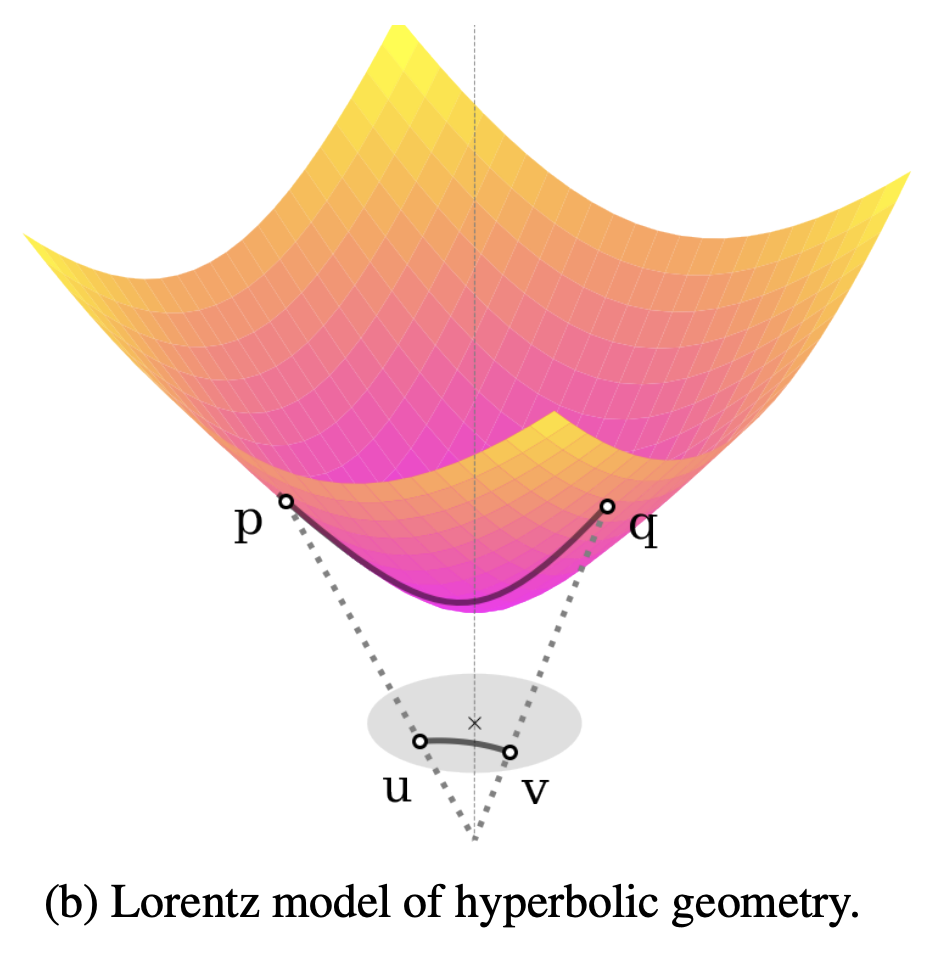
\includegraphics[width=0.4\textwidth]{lectures/11-b/Images/1-Lorentz.png}
    \caption{Lorentz model of hyperbolic geometry}
    \label{fig:1-Lorentz}
\end{figure}

But the problem with this is that the optimization is sometimes tricky to get right so people often resort to using small batch sizes, which results in slow convergence and the model will get stuck in local mini-ma. One way to improve these tools is to develop optimization methods in many manifolds that work significantly better than what we have now.

The Lorentz model in figure (~\ref{fig:1-Lorentz}) proposed by (Nickel et. al., 2018) showed good improvements over the Poincare disk. And advanced methods such as the RSVRG proposed by (Zhang et. al., 2016) didn't show significant gains for embeddings.  

\subsection{Methods}

Another important thing to think about conceptually is that if we switch the geometry, we now can not use easily our standard machine learning to do the task. A lot of benefits that we typically have from embedding is that they are intrinsic to relation-learning. Take word embeddings for example. The problem is that the standard machine learning, especially deep learning frameworks they all make this assumption. So you can't expect to just put the embeddings in and expect them to do something. So how can we make these embeddings usable? Is there some kind of translation we can adapt.

Researchers have found that using Riemannian manifolds in latent spaces for generative models is very promising as explored by Davidson et. al., 2018, as shown in figure (~\ref{fig:2-Davidson}). However, they have also been widely used in natural language understanding in downstream tasks. But a majority of machine learning and deep learning makes the Euclidean assumption.

\begin{figure}[htb]
  \centering
    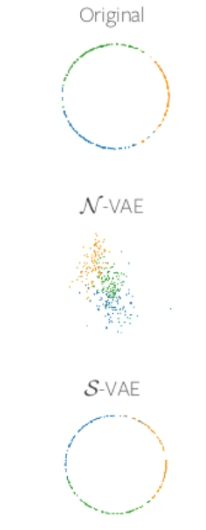
\includegraphics[width=0.2\textwidth]{lectures/11-b/Images/2-Davidson.png}
    \caption{Riemannian manifolds for generative models is very promising}
    \label{fig:2-Davidson}
\end{figure}

\subsection{Embedding and Cognitive Science}

In cognitive science, the human similarity judgments are often non-metric. The classic example is that if you ask a human whether a man is similar to a centaur as depicted in figure (~\ref{fig:3-cog}), they will say yes. And if ask a human whether a centaur is similar to a horse, they will also say yes. However, if we ask a human whether a horse is similar to a man, they will say no. And it is a very strongly no. The problem with this is that if we have a very strong disagreement in these similarity judgments, it conflicts with the triangle inequality, which says: 

\begin{equation} \label{eq:triangleIne}
    d(u,v) \leq d(u, w) + d(w, v)
\end{equation}

This means that we won't be able to embed these similarity judgments properly. In this case, we need to think about non-metric measures. But this opens another can of worms.

\begin{figure}[htb]
  \begin{center}
    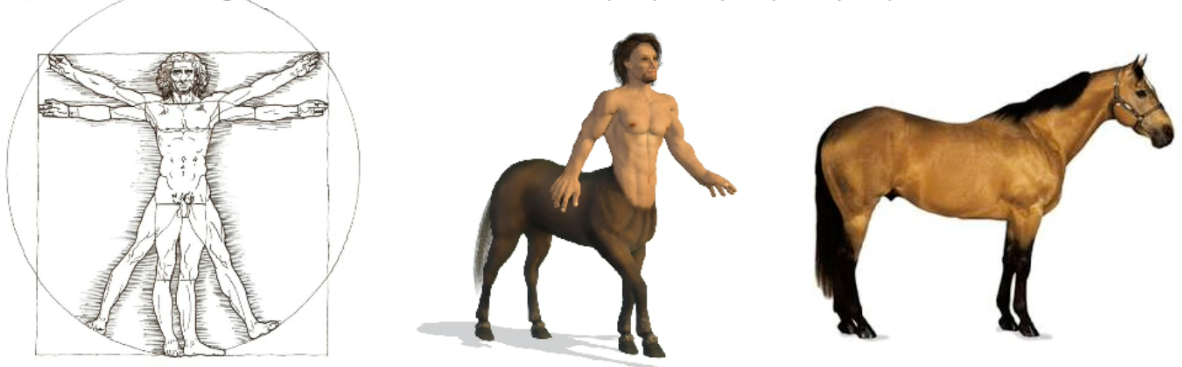
\includegraphics[width=0.8\textwidth]{lectures/11-b/Images/3-cog.png}
    \caption{The human similarity judgment experiment in cognitive science}
    \label{fig:3-cog}
    \end{center}
\end{figure}

\subsection{Tools}

Hype is an open source library to embed graphs into hyperbolic space. It can be used to play with these models. It is a Pytorch-based embeddings framework and supports Hyperbolic, Euclidean and Spherical manifolds. It is available on github via the following link:

http://github.com/facebookresearch/poincare-embeddings.


\section{Summary}

Christopher Strachey in a letter to Alan Turing summarized the utilization of relations  between data entities and their applications to Logical, analogical, taxonomical and knowledge bases.


\begin{itemize}
    \item Relational embeddings provide high-quality models of large-scale relational data.
    \item Graph neural networks learn inductive models of graph-structured data.
    \item Geometry of the embedding space acts as a prior on the structure of similarity relations.
    \item Hyperbolic embeddings are used to capture similarity and hierarchy in symbolic data
\end{itemize}
